% ==============================================================================
\section{Módulo de visión}
\label{sec:dev_vision}
% ==============================================================================

\subsection{Descripción}

El módulo de visión recibe cada cuadro de la cámara y entrega una lista de
detecciones. Para cada objeto se indica qué es, en qué dirección está respecto al frente
del usuario, a qué distancia aproximada se encuentra, si se está moviendo y, en el caso
de las puertas, si está abierta o cerrada. Con esa lista trabajan el SLAM, las alertas y
la descripción del entorno que el usuario puede pedir por voz. El módulo atiende los
requerimientos RF-07 a RF-10 y RF-13.

En TT1 el módulo se planteó alrededor de un solo detector, YOLOv8. Al probarlo con los
videos reales salió a la luz su mayor carencia, pues el conjunto COCO con el que viene
entrenado no incluye puertas, escaleras ni escritorios, que son justamente los objetos
que más ayudan a orientarse dentro de un edificio. Por eso la versión final combina tres
modelos preentrenados, cada uno con una tarea distinta, como se resume en la
Tabla~\ref{tab:vision_modelos}.

\begin{table}[H]
\centering
\caption{Modelos que componen el módulo de visión}
\label{tab:vision_modelos}
\renewcommand{\arraystretch}{1.25}
\begin{tabular}{|p{3.4cm}|p{3.1cm}|p{2.3cm}|p{5.7cm}|}
\hline
\textbf{Modelo} & \textbf{Entrenamiento} & \textbf{Frecuencia} & \textbf{Uso} \\
\hline
YOLOv8s-seg & COCO, 80 clases & Cada cuadro & Personas, vehículos, muebles y objetos
comunes \cite{redmon2016yolo}. \\
\hline
YOLOv8s & Open Images V7, 600 clases & Cada 5 cuadros (15 en la Raspberry Pi) & Solo
las clases que COCO no tiene, como puerta, escalera, ventana, bote de basura, poste,
letrero, árbol, escritorio, archivero o pizarrón. \\
\hline
SegFormer-B0 & ADE20K, 150 clases & Cada 4 a 10 cuadros & Segmentación de la escena
para encontrar piso transitable, agua, escaleras y puertas \cite{xie2021segformer,
zhou2017ade20k}. \\
\hline
\end{tabular}
\end{table}

\subsection{Preprocesamiento y geometría de la cámara}

Cada cuadro se reduce a 640 píxeles de ancho conservando su relación de aspecto. Una
versión anterior lo forzaba a $640 \times 480$; en los videos 16:9 eso estiraba la
imagen en vertical, inflaba la altura de las cajas y hacía que las distancias salieran
cerca de un 25\,\% más cortas. Ahora la dirección, la distancia por altura típica y la
distancia por plano de piso se calculan con una sola distancia focal, obtenida del campo
de visión horizontal. Hay dos perfiles de cámara, uno para la cámara web de la
computadora portátil ($70^\circ$) y otro para la Camera Module 3 Wide del prototipo
($102^\circ$). Las ecuaciones de distancia se presentan en la Sección~\ref{sec:dev_slam};
el rango estimado se acota entre 0.2 y 8~m.

La igualación de histograma y el filtro gaussiano del pseudocódigo de TT1
(Apéndice~\ref{apend:procesa}) se dejaron fuera. Los modelos preentrenados ya normalizan
la imagen por dentro y, en las pruebas con video, esos pasos no mejoraron nada que
justificara su costo por cuadro.

\subsection{Detección de objetos}

El detector principal es YOLOv8s-seg con un umbral de confianza de 0.45. Algunas
etiquetas de COCO se renombran para que coincidan con el resto del sistema (por ejemplo,
\emph{couch} pasa a \emph{sofa} y \emph{tv} a \emph{monitor}). El detector de Open
Images se ejecuta con un umbral de 0.25 y solo cada cierto número de cuadros, porque en
CPU cuesta casi lo mismo que el principal. De sus 600 clases se conservan nada más las
que aportan algo nuevo, y si una de sus cajas se encima con una de COCO con un IoU mayor
a 0.55, se descarta para no contar dos veces el mismo objeto. La lista de clases creció
después de una prueba en la sala de maestros de la escuela, donde el sistema casi no
detectaba nada porque los escritorios y archiveros no existían en COCO.

\subsection{Puertas, piso y peligros por segmentación}

SegFormer asigna una clase a cada píxel de la imagen, y de ese mapa se sacan tres tipos
de información. La primera son las puertas. Cada región conexa de la clase puerta que
ocupa al menos el 0.4\,\% de la imagen se convierte en una detección, y se considera
abierta si dentro de su recuadro hay más de un 7\,\% de piso transitable, es decir, si a
través del vano se alcanza a ver el piso del otro lado. Cuando el detector de Open
Images ya vio una puerta en la misma dirección (con menos de $8^\circ$ de diferencia),
se conserva solo una. Además, si la puerta queda dentro del haz de los ultrasónicos, el
eco decide su estado, como se explica en la Sección~\ref{sec:dev_slam}.

La segunda son el agua y las escaleras, que ADE20K reconoce como clases propias. Se
toman las regiones que aparecen en el 55\,\% inferior de la imagen y se ubican con la
distancia por plano de piso. La tercera son los hoyos y coladeras, para los que no
existe una clase. Se detectan como regiones no transitables rodeadas de piso, con
varias condiciones para evitar confusiones; la región debe estar en la parte baja de la
imagen, ocupar entre el 0.15 y el 20\,\% del cuadro, no tocar los bordes y estar rodeada
de piso transitable en al menos un 55\,\% de su contorno. Si un peligro coincide en
dirección y distancia con un objeto que ya detectó YOLO, se descarta, porque casi
siempre se trata de la sombra o la base de ese mismo objeto.

\subsection{Objetos en movimiento}

El rastreador de \texttt{vision/motion.py} asocia las cajas entre cuadros y guarda el
historial de sus centroides; si un objeto se desplaza más de 8 píxeles, se marca como
móvil. Las personas, los animales y los vehículos se marcan siempre como móviles. En la
primera versión, cada vez que el usuario giraba la cabeza todo el cuarto parecía
moverse. Para corregirlo, antes de comparar se desplaza el historial del rastreador lo
que corresponde al giro medido por la odometría, $\Delta u = \Delta\theta \cdot W /
\text{FOV}_h$, y así solo queda el movimiento propio de los objetos.

\subsection{Nivel de riesgo}

Cada detección recibe un nivel de riesgo de 0 a 3 según la tabla definida en TT1
(Tabla~\ref{tabla_riesgo}). Los peligros de piso y los objetos en movimiento tienen
riesgo alto (3), los obstáculos estáticos y las puertas cerradas riesgo medio (2), y las
puertas abiertas y las paredes riesgo bajo (1). El mapeo agrupa estos niveles por sector
para construir $r_{\text{front}}$, $r_{\text{left}}$ y $r_{\text{right}}$.

\subsection{Resultados}

La Figura~\ref{fig:vision_escenas} muestra el módulo trabajando sobre tres escenas de
los videos reales. A la izquierda se marcan las detecciones con su distancia estimada
(en verde los objetos estáticos, en rojo los móviles y en magenta los peligros de piso)
y a la derecha la segmentación, con el piso transitable en verde, las puertas en azul y
las paredes en gris.

\begin{figure}[H]
    \centering
    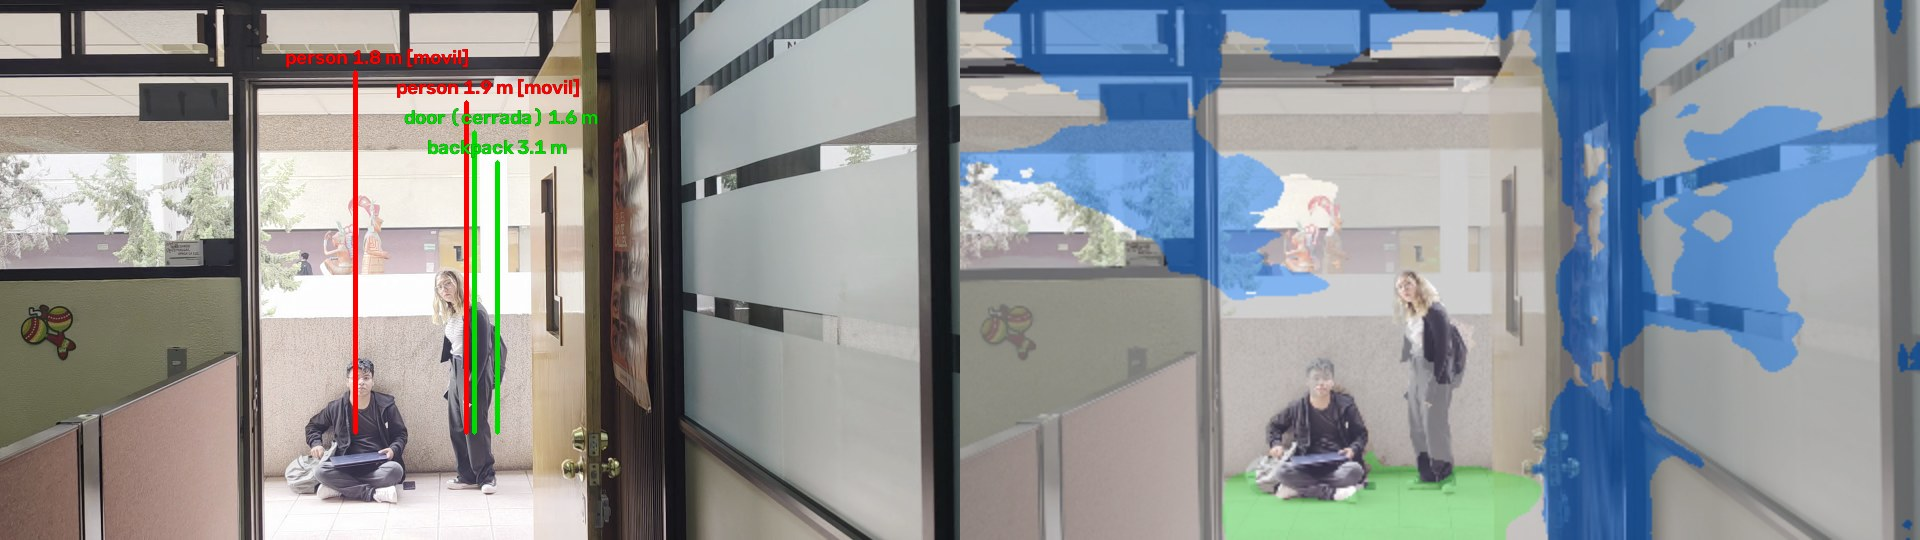
\includegraphics[width=\textwidth]{Capturas_TT2/vision/vision_escena11.jpg}\\[2pt]
    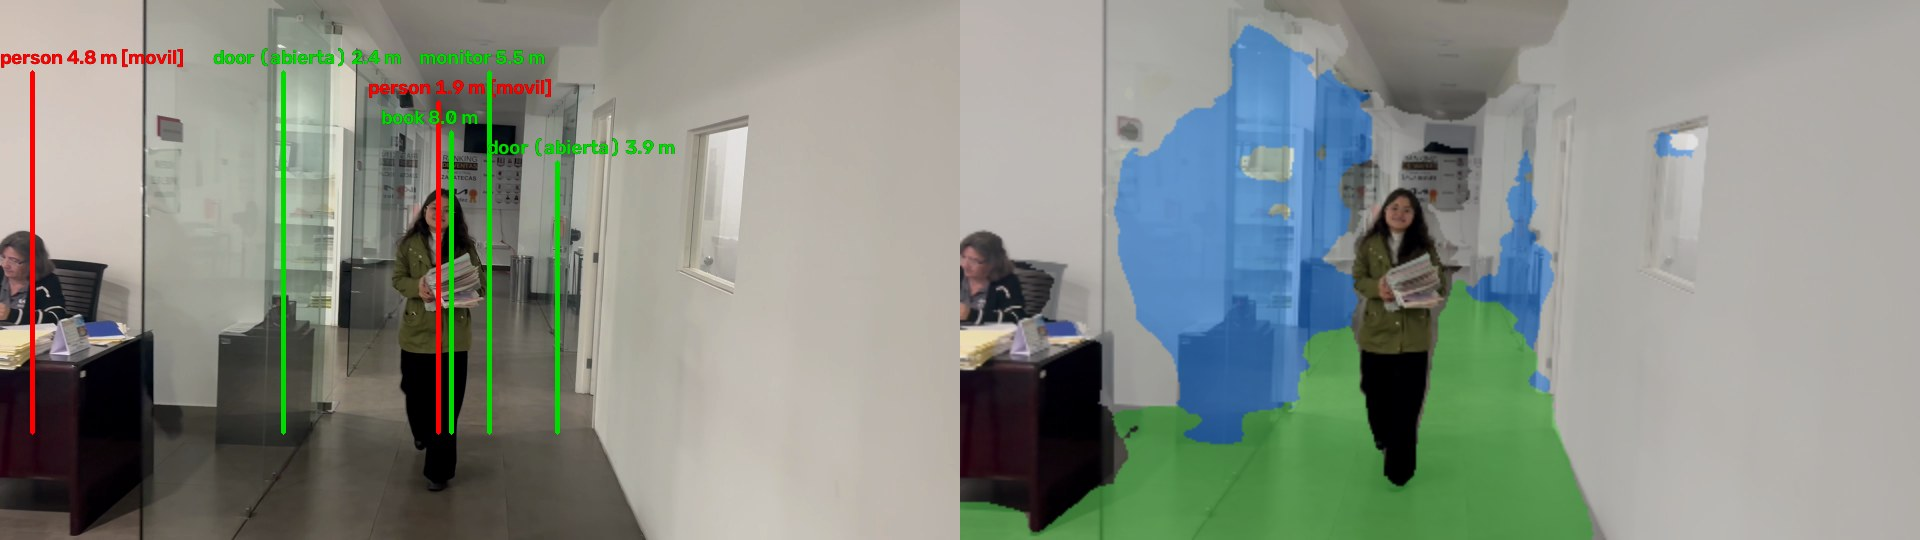
\includegraphics[width=\textwidth]{Capturas_TT2/vision/vision_escena14.jpg}\\[2pt]
    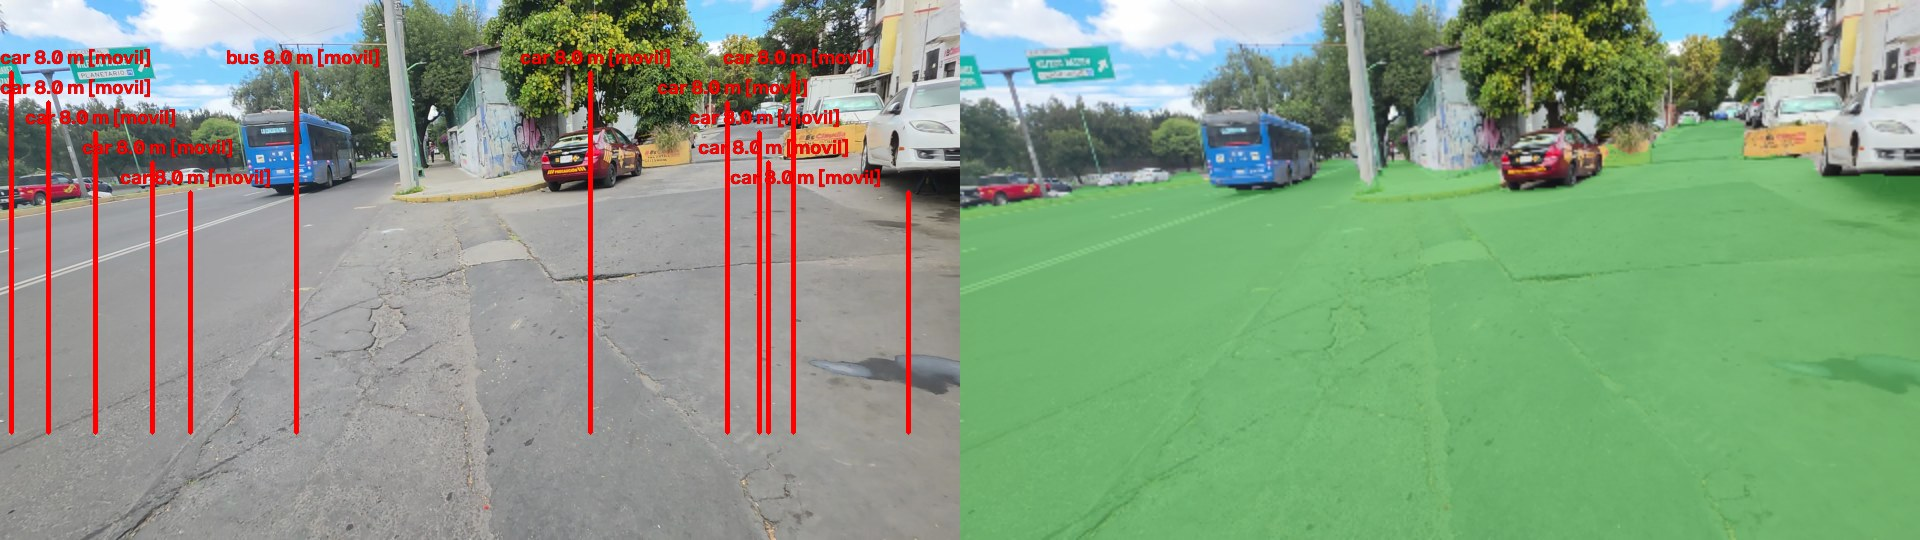
\includegraphics[width=\textwidth]{Capturas_TT2/vision/vision_escena6.jpg}
    \caption{Detecciones (izquierda) y segmentación (derecha) en la entrada de la sala
    de maestros, en un pasillo de oficina con una persona caminando y en una calle con
    vehículos.}
    \label{fig:vision_escenas}
\end{figure}

En la entrada de la sala de maestros el sistema detecta a las dos personas, una mochila
y la puerta, que clasifica como cerrada a 1.6~m. En el pasillo de oficina detecta a la
persona que camina hacia la cámara (a 1.9~m), un monitor y dos puertas abiertas, aunque
la segmentación también marca como puerta buena parte de los canceles de vidrio, así que
al menos una de esas ``puertas'' es en realidad una mampara. La señora sentada en el
escritorio aparece a 4.8~m cuando está a unos 2~m; la distancia se calcula con la altura
típica de una persona de pie (1.65~m), y alguien sentado se ve más bajo, lo que el
modelo interpreta como lejanía. En la calle, los vehículos aparecen como móviles y a
8~m, que es el tope del rango. Más delicado es que la segmentación pinta como piso
transitable tanto la banqueta como el arroyo vehicular, porque la clase \emph{road} de
ADE20K está entre las superficies transitables, y que los baches del pavimento no se
reportan como peligro.

La Figura~\ref{fig:vision_tapete} muestra un falso positivo típico. Un tapete con un
estampado oscuro sobre un piso claro cumple todas las condiciones de un hoyo, porque la
segmentación no lo reconoce como piso, está en la parte baja de la imagen y tiene piso
alrededor. El sistema lo reporta como hoyo a 0.9~m.

\begin{figure}[H]
    \centering
    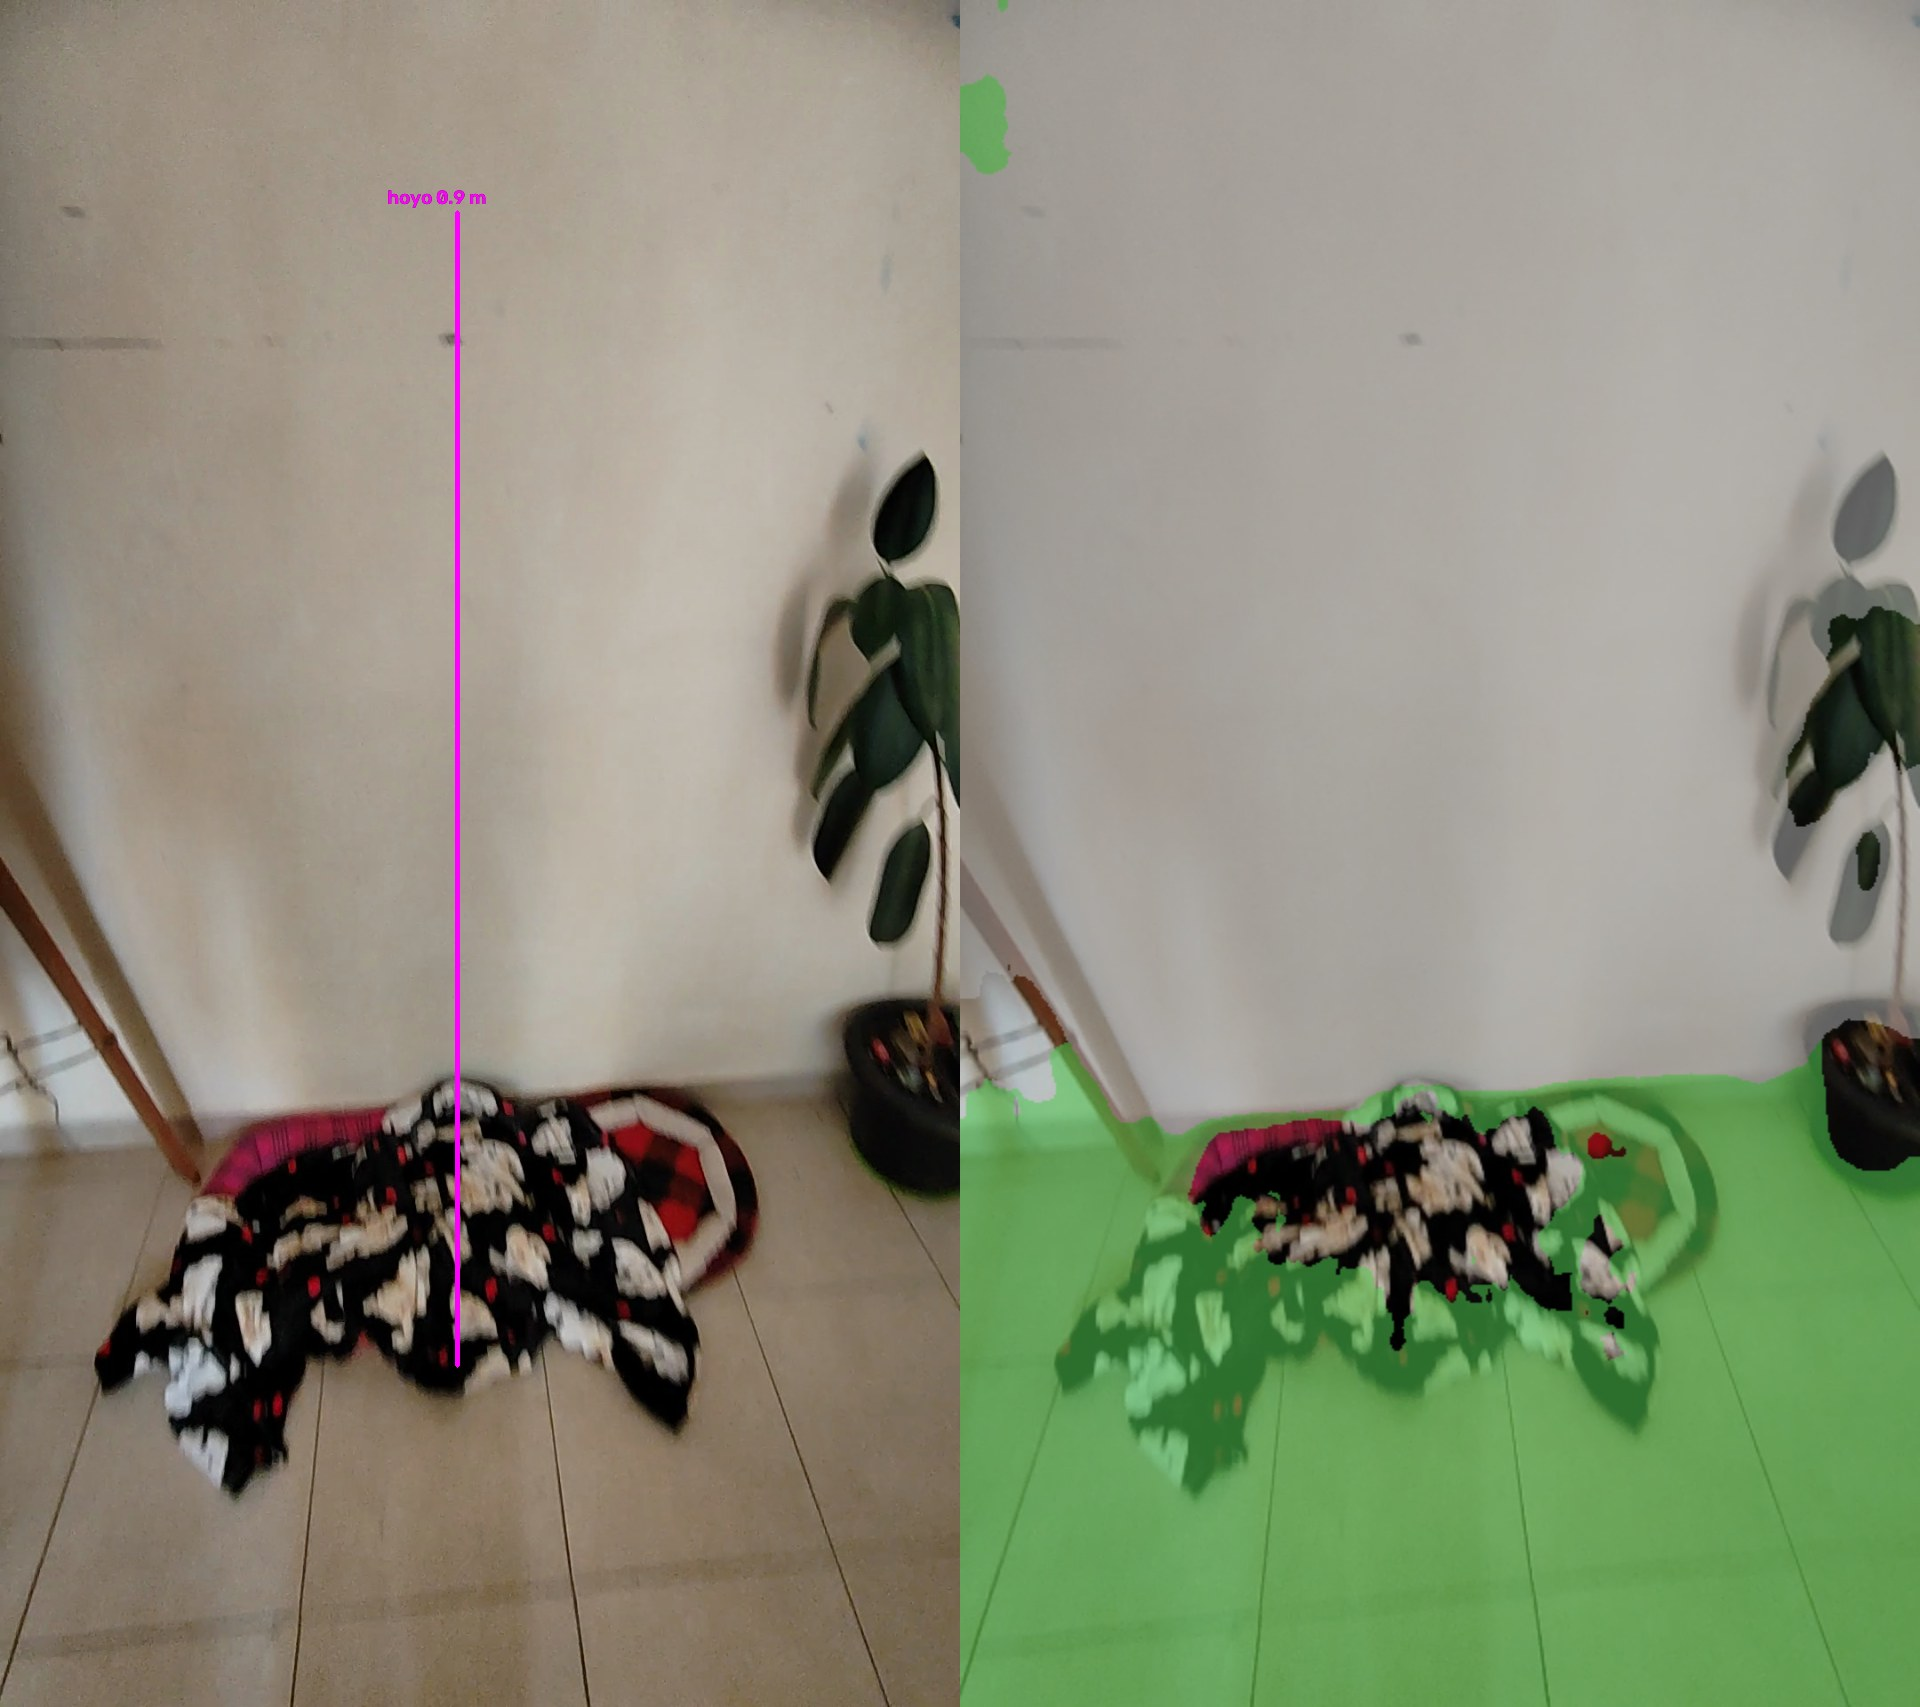
\includegraphics[width=0.62\textwidth]{Capturas_TT2/vision/vision_escena16.jpg}
    \caption{Falso positivo: un tapete estampado se detecta como hoyo a 0.9~m.}
    \label{fig:vision_tapete}
\end{figure}

La Tabla~\ref{tab:vision_tiempos} reporta el tiempo de inferencia de cada modelo,
medido en CPU sobre el mismo cuadro, en la computadora portátil y en la Raspberry Pi del
prototipo.

\begin{table}[H]
\centering
\caption{Tiempo de inferencia por modelo (promedio de 10 ejecuciones)}
\label{tab:vision_tiempos}
\renewcommand{\arraystretch}{1.2}
\begin{tabular}{|l|c|c|c|}
\hline
\textbf{Modelo} & \textbf{Entrada} & \textbf{Apple M4 (ms)} &
\textbf{Raspberry Pi (ms)} \\
\hline
YOLOv8s-seg (COCO) & $640 \times 360$ & 72 & \TODO{} \\
YOLOv8s (Open Images V7) & $640 \times 360$ & 55 & \TODO{} \\
SegFormer-B0 con puertas y peligros & $480 \times 270$ & 293 & \TODO{} \\
\hline
\end{tabular}
\end{table}

En la computadora portátil, con el detector principal en cada cuadro, el extra cada
cinco y la segmentación cada cuatro, el costo promedio es de unos 160~ms por cuadro, o
sea, unos 6 cuadros por segundo. La segmentación es lo más caro; por eso se ejecuta con
menos frecuencia y sus resultados se reutilizan en los cuadros intermedios. En la
Raspberry Pi, con la configuración del prototipo (extra cada 15 cuadros y segmentación
cada 10), el sistema procesa \TODO{cuadros por segundo en la Raspberry Pi}.

La precisión de detección que pide RNF-06 se mide sobre imágenes tomadas con la
cámara del prototipo y etiquetadas a mano. \TODO{armar el conjunto y reportar número de
imágenes, clases, precisión y exhaustividad}. Para mejorar las clases propias del
entorno se cuenta con el script \texttt{vision/finetune.py}, que reentrena YOLO con un
conjunto en formato YOLO. \TODO{resultado del reentrenamiento con puertas y mamparas de
la escuela, si se realiza}. El módulo tiene 15 pruebas automatizadas que usan detectores
simulados para revisar la geometría, las puertas, el detector extra y la eliminación de
duplicados.

\subsection{Limitaciones}

Ninguno de los tres modelos tiene una clase para mamparas o canceles de vidrio. La
segmentación a veces los toma por puertas y a veces no los ve; los ultrasónicos
frontales compensan en parte, porque un eco sin detección visual se avisa como pared y
el eco corrige el estado de las puertas de vidrio, pero solo dentro de su cono angosto.
El criterio geométrico de los hoyos también genera falsos positivos con tapetes,
manchas y cambios de textura del piso.

El rastreador compensa el giro del usuario, pero no su avance. Al caminar hacia
adelante, las cajas de los objetos cercanos crecen y algunos objetos estáticos se marcan
como móviles, como se ve en la Figura~\ref{fig:cap_oficina_3}. La distancia monocular,
por su parte, depende de la altura típica de cada clase, de modo que una persona sentada
o un objeto de tamaño poco común quedan mal ubicados, y se satura en 8~m. Por último, la
calle se considera tan transitable como la banqueta y los baches poco profundos no se
distinguen del pavimento, así que en exteriores el sistema no sabe por sí solo que bajar
al arroyo vehicular es peligroso. \TODO{separar banqueta y arroyo vehicular en la
segmentación}.
